\documentclass[10pt,a4paper]{report}
\newcommand{\confdir}{../conf/} % Set the folder which contains preamble.tex, titlepage.tex and the general img/ folder
\newcommand{\imgdir}{img/} % Set the folder which contains the specific images for the report
\newcommand{\texdir}{tex/} % Set the folder which contains the content (.tex files)
\input{\confdir preamble}


%%%%%%%%%%%
%% SETUP %%
%%%%%%%%%%%

%% Set the course number and course name
% Usage: \setcourse{<course no>}{<course name>}
	\setcourse{02450}{Introduction to Machine Learning and Data Modeling}

%% Set the title of the report
% Usage: \settitle{<title>}
	\settitle{Assignment 1}

%% Set the subtitle of the report
% Usage: \setsubtitle{<subtitle>}
	\setsubtitle{Feature Extraction and Visualization}

%% Set the date the report is handed in
% Usage: \setdate{<hand-in date>}
	\setdate{March 5th 2013}

%% Add the authors of the report
% Usage: \addauthor{<study number>}{<first name(s)>}{<last name>}
	\addauthor{s093294}{Poul Kjeldager}{Sørensen}
	\addauthor{s093280}{Martin Kasban}{Tange}

%%%% END OF SETUP

%ADDED BY POUL
\renewcommand{\topfraction}{0.85}
\renewcommand{\textfraction}{0.1}
\renewcommand{\floatpagefraction}{0.75}
\usepackage[draft,english,margin]{fixme}




\begin{document}

%% Insert titlepage
\inserttitlepage

%% Insert table-of-contents
\inserttoc

%% Input files for the report
\input{\texdir introduction}
\chapter{Data and Feature Extraction}
\section{Introduction}
\fixme{Write about where the data are from and the feature extraction method.}

\chapter{Data Analysis}
\section{Introduction}
Introduce what this chapter is about.
\section{Basic Statistic Properties}
Show the basic statistics properties of the dataset.
\begin{figure}[hbtp]
\begin{minipage}[b]{.45\linewidth}
\centering\large A
\subcaption{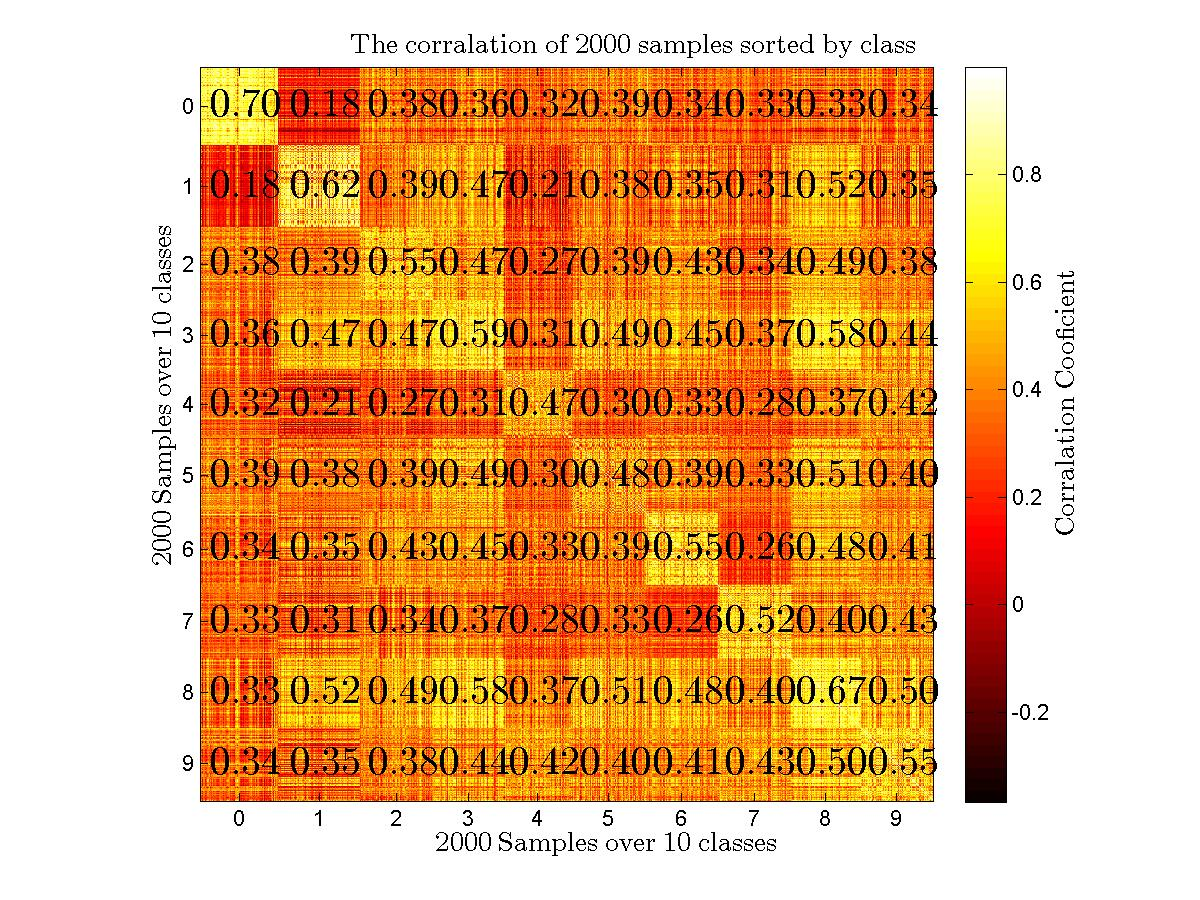
\includegraphics[width=\linewidth]{corr_explained}}\label{fig:1a}
\end{minipage}%
\hfill
\begin{minipage}[b]{.45\linewidth}
\centering\large B

\subcaption{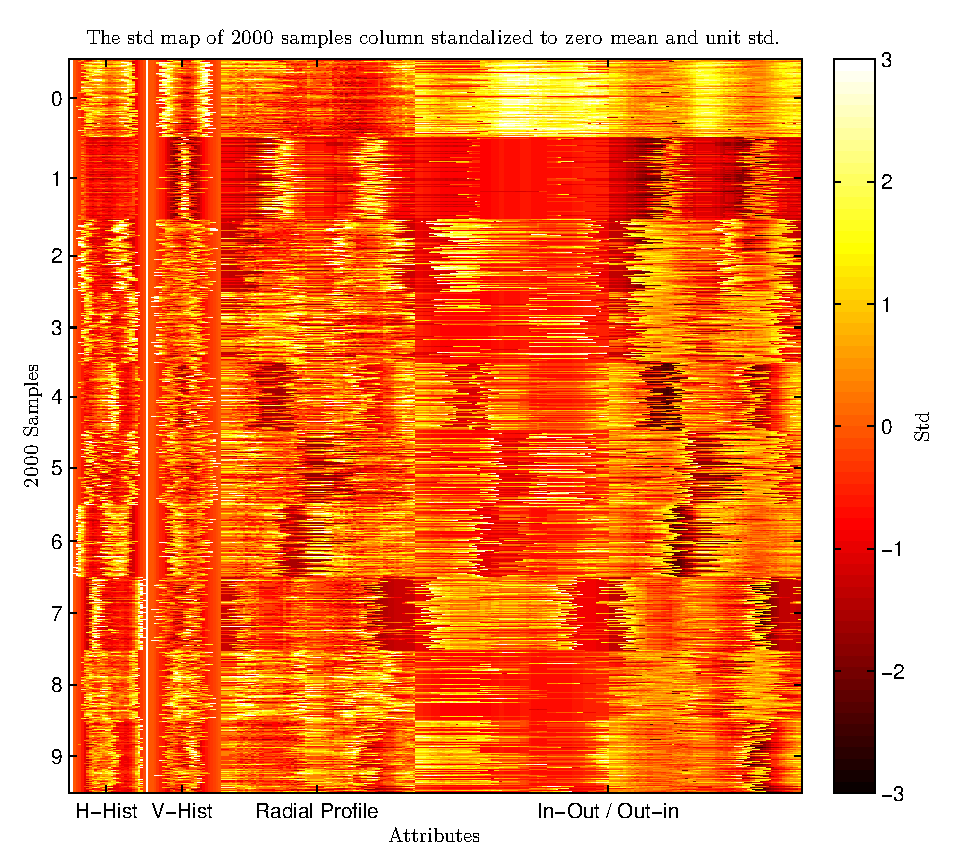
\includegraphics[width=\linewidth]{std_explained}}\label{fig:1b}
\end{minipage}
\caption{A figure}\label{fig:1}
\end{figure}

\subsection{Correlation}
Talk about correlation and explain Figure~\ref{fig:1a}.



\section{Principal Component Analysis}
\fixme{The amount of variation explained as a function of the number of PCA com- ponents included}
\fixme{the principal directions of the considered PCA components}
\fixme{the data projected onto the considered principal components}
\input{\texdir pca}

\chapter{Discussion}

\section{Conclusion}



\end{document}
